
\chapter{Atomo di Idrogeno}

\lezione{1}{23/02/2026}

\section{Elementi essenziali}

L''analisi dell'atomo idrogenoide costituisce il punto di partenza fondamentale per lo studio della struttura atomica nella meccanica quantistica moderna. 
Per atomo idrogenoide si intende un sistema legato composto da un nucleo di carica elettrica $+Ze$ (dove $Z$ è il numero atomico) e da un singolo elettrone di carica $-e$.


\subsection{Descrizione quantistica}

Consideriamo l'Hamiltoniano imperturbato di un atomo isolato, definito dalla somma dell'energia cinetica ($T$) e del potenziale ($V$):
\begin{equation}
    H^{(0)} = H_{(0)} = T + V
\end{equation}

Il sistema descrive un nucleo di carica $+Ze$ e un elettrone di carica $-e$. Introduciamo le seguenti variabili nel sistema di riferimento del laboratorio (SR LAB):
\begin{itemize}
    \item $M_N$: massa del nucleo;
    \item $m_e$: massa dell'elettrone;
    \item $\vec{R}_N$: posizione del nucleo;
    \item $\vec{r}_e$: posizione dell'elettrone.
\end{itemize}

\begin{figure}[htbp]
    \centering
    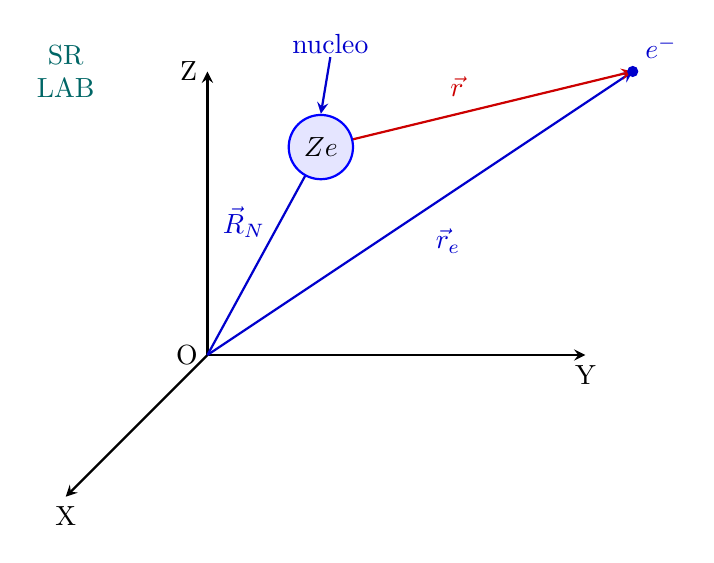
\begin{tikzpicture}[>=stealth, scale=1.2]
        
        % Assi cartesiani (SR LAB)
        \draw[->, thick] (0,0) -- (0,3) node[left] {Z};
        \draw[->, thick] (0,0) -- (4,0) node[below] {Y};
        \draw[->, thick] (0,0) -- (-1.5,-1.5) node[below] {X};
        \node[left] at (0,0) {O};
        \node[color=teal!80!black, align=center] at (-1.5,3) {SR\\LAB};

        % Coordinate dei punti
        \coordinate (N) at (1.2, 2.2); % Posizione Nucleo
        \coordinate (E) at (4.5, 3.0); % Posizione Elettrone

        % Vettori posizione dal SR LAB (in blu)
        \draw[->, thick, blue!80!black] (0,0) -- (N) node[midway, above left =1pt, xshift = 5pt] {$\vec{R}_N$};
        \draw[->, thick, blue!80!black] (0,0) -- (E) node[midway, below right=2pt] {$\vec{r}_e$};

        % Vettore distanza relativa (in rosso)
        \draw[->, thick, red!80!black] (N) -- (E) node[midway, above left=1pt] {$\vec{r}$};

        % Disegno Nucleo
        \node[circle, draw=blue, fill=blue!10, thick, minimum size=8mm] (nucleo_node) at (N) {$Ze$};
        \draw[<-, blue!80!black, thick] (nucleo_node.north) -- ++(0.1,0.6) node[above, inner sep=1pt] {nucleo};

        % Disegno Elettrone
        \filldraw[blue!80!black] (E) circle (1.5pt) node[above right=1pt] {$e^-$};
        
    \end{tikzpicture}
    \caption{Coordinate spaziali dell'atomo isolato rispetto al sistema di riferimento del laboratorio (SR LAB).}
    \label{fig:coordinateLAB_atomo}
\end{figure}

L'espressione esplicita dell'Hamiltoniano è:
\begin{equation}
    H^{(0)} = -\frac{\hbar^2}{2M_N} \nabla_{R_N}^2 - \frac{\hbar^2}{2m_e} \nabla_{r_e}^2 - \frac{Ze^2}{4\pi\epsilon_0} \frac{1}{|\vec{r}_e - \vec{R}_N|}
\end{equation}

La funzione d'onda totale $\Psi_E^{(0)}(\vec{r}_e, s, \vec{R}_N, t)$ soddisfa l'equazione di Schrödinger dipendente dal tempo:
\begin{equation}
    i\hbar \pdv{t} \Psi_E^{(0)} = H^{(0)} \Psi_E^{(0)}
\end{equation}

Trattandosi di un sistema stazionario, separiamo la dipendenza temporale tramite l'autovalore dell'energia $E^{(0)}$ associato a $H^{(0)}$:
\begin{equation}
    \Psi_E^{(0)} = \Psi_E^{(0)}(\vec{r}_e, s, \vec{R}_N) e^{-\frac{i}{\hbar}E^{(0)}t}
\end{equation}
In questa formulazione, la funzione d'onda comprende una parte spaziale, una parte di spin ($s$) e la componente temporale.

Poiché l'Hamiltoniano $H^{(0)}$ non dipende dalle variabili di SPIN, possiamo fattorizzare la soluzione:
\begin{tcolorbox}[colback=blue!5, colframe=blue!50, sharp corners, boxrule=0.5pt]
    \begin{equation}
        \Psi_E^{(0)} = \psi_E^{(0)}(\vec{r}_e, \vec{R}_N) \chi(s) e^{-\frac{i}{\hbar}E^{(0)}t}
    \end{equation}
\end{tcolorbox}

Dove:
\begin{itemize}
    \item $\chi(s)$ rappresenta l'autofunzione di SPIN;
    \item $\psi_E^{(0)}(\vec{r}_e, \vec{R}_N)$ rappresenta l'autofunzione SPAZIALE.
\end{itemize}

L'equazione agli autovalori per la componente spaziale è dunque:
\begin{equation}
    H^{(0)} \psi_E^{(0)}(\vec{r}_e, \vec{R}_N) = E^{(0)} \psi_E^{(0)}(\vec{r}_e, \vec{R}_N)
\end{equation}

\subsubsection{Soluzione equazione spaziale}
Per risolvere l'equazione agli autovalori conviene cambiare sistema di riferimento (SR). Passiamo al sistema di riferimento del centro di massa (SR CM) utilizzando le coordinate sferiche, poiché per i problemi a due corpi il SR CM risulta il più comodo per i calcoli.

Definiamo le variabili del sistema nel centro di massa:
\begin{itemize}
    \item Posizione del Centro di Massa: $\vec{R}_{CM} = \frac{m_e \vec{r}_e + M_N \vec{R}_N}{m_e + M_N} \approx \vec{R}_N$
    \item Massa ridotta: $\mu = \frac{M_N m_e}{m_e + M_N} \approx m_e$
    \item Massa totale: $M_{TOT} = m_e + M_N$
\end{itemize}

Introducendo la coordinata relativa $\vec{r} = \vec{r}_e - \vec{R}_N$, l'Hamiltoniano diventa:
\begin{equation}
    H^{(0)} = -\frac{\hbar^2}{2M_{TOT}} \nabla_{R_{CM}}^2 - \frac{\hbar^2}{2\mu} \nabla_{r}^2 - \frac{Ze^2}{4\pi\epsilon_0 r}
\end{equation}

Trascurando l'energia cinetica del nucleo (ovvero assumendo il nucleo infinitamente pesante rispetto all'elettrone), otteniamo l'Hamiltoniano approssimato:
\begin{equation}
    H^{(0)} \approx -\frac{\hbar^2}{2\mu} \nabla_{r}^2 - \frac{Ze^2}{4\pi\epsilon_0 r}
\end{equation}


Esprimiamo il vettore posizione relativa $\vec{r} = (x, y, z)$ in coordinate sferiche. Se passiamo in sferiche, le relazioni di trasformazione sono:
\begin{equation}
    \begin{cases}
        x = r \sin\theta \cos\phi \\
        y = r \sin\theta \sin\phi \\
        z = r \cos\theta
    \end{cases}
\end{equation}
\begin{figure}[htbp]
    \centering
    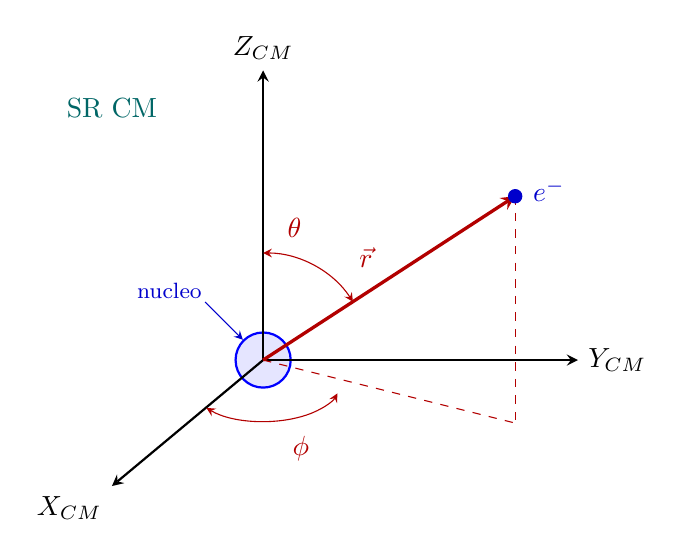
\begin{tikzpicture}[>=stealth, scale=1.6]
    % Definizione dell'origine (Centro di Massa)
    \coordinate (O) at (0,0);
    
    % 1. Disegno del Nucleo all'origine
    % Disegnato per primo così non copre le linee degli assi e del vettore
    \node[circle, draw=blue, fill=blue!10, thick, minimum size=7mm] (nucleo) at (O) {};
    \draw[<-, blue!80!black, thin] (nucleo.north west) -- ++(-0.3,0.3) node[above left, inner sep=1pt] {\footnotesize nucleo};

    % Assi coordinati (fissi per garantire stabilità visiva)
    \draw[->, thick] (O) -- (0,2.3) node[above] {$Z_{CM}$}; % Asse Z verticale
    \draw[->, thick] (O) -- (2.5,0) node[right] {$Y_{CM}$}; % Asse Y orizzontale
    \draw[->, thick] (O) -- (-1.2,-1.0) node[below left] {$X_{CM}$}; % Asse X diagonale
    
    \node[color=teal!80!black, align=center] at (-1.2,2) {SR CM};

    % Punto P (la punta del vettore r) e la sua proiezione sul piano XY
    \coordinate (P) at (2.0, 1.3); 
    \coordinate (Pproj) at (2.0, -0.5);

    % Linee di proiezione tratteggiate
    \draw[dashed, red!70!black] (P) -- (Pproj);
    \draw[dashed, red!70!black] (O) -- (Pproj);

    % Vettore posizione r (in rosso scuro/marrone come da foto)
    \draw[->, very thick, red!70!black] (O) -- (P) node[midway, above left, xshift=-2pt] {$\vec{r}$};

    % Angolo theta (tra l'asse Z e il vettore r)
    \draw[red!70!black, <->] (0,0.85) arc (90:33:0.85);
    \node[red!70!black] at (0.25, 1.05) {$\theta$};

    % Angolo phi (tra l'asse X e la proiezione sul piano XY)
    \draw[red!70!black, <->] (-0.45,-0.38) arc (220:345:0.6 and 0.3);
    \node[red!70!black] at (0.3, -0.7) {$\phi$};

    % 2. Disegno dell'Elettrone al punto P
    % Disegnato per ultimo così copre la punta della freccia rossa
    \filldraw[blue!80!black] (P) circle (1.5pt) node[right=3pt, yshift=2pt] {$e^-$};

\end{tikzpicture}
    \caption{Coordinate spaziali dell'atomo isolato rispetto al sistema di riferimento del centro di massa (SR CM).}
    \label{fig:coordinateCM_atomo}
\end{figure}

L'operatore Laplaciano $\nabla_r^2$ può essere riscritto in coordinate sferiche $(r, \theta, \phi)$ per facilitare la risoluzione dell'equazione agli autovalori:
\begin{equation}
    H^{(0)} \psi_E^{(0)}(\vec{r}_e, \vec{R}_N) = E^{(0)} \psi_E^{(0)}(\vec{r}_e, \vec{R}_N)
\end{equation}
Esprimendo il sistema in termini delle coordinate del centro di massa $\vec{R}_{CM}$ e della posizione relativa $\vec{r} = \vec{r}_e - \vec{R}_N$, l'Hamiltoniano completo assume la forma:

\begin{equation}
    H^{(0)} = \underbrace{\left\{ -\frac{\hbar^2}{2\mu} \frac{1}{r^2} \pdv{r} \left( r^2 \pdv{r} \right) + \frac{L^2}{2\mu r^2} - \frac{Ze^2}{4\pi\epsilon_0 r} \right\}}_{\text{Parte relativa}} \underbrace{- \frac{\hbar^2}{2M_{TOT}} \nabla_{R_{CM}}^2}_{\text{Parte CM}}
\end{equation}

Introduciamo l'operatore momento angolare orbitale $\vec{L}$. Data la simmetria del problema, l'Hamiltoniano commuta con gli operatori $L^2$ e $L_z$:
\begin{equation}
    [H^{(0)}, L^2] = 0, \quad [H^{(0)}, L_z] = 0
\end{equation}
È quindi possibile scegliere una base comune di autofunzioni per questi tre osservabili.

Nel sistema di riferimento del centro di massa e in coordinate sferiche, per stati legati ($E \le 0$), la soluzione $\psi_E^{(0)}(\vec{r}, \vec{R}_{CM})$ si fattorizza nel prodotto di una componente radiale e una angolare:
\begin{tcolorbox}[colback=blue!5, colframe=blue!50, sharp corners, boxrule=0.5pt]
    \begin{equation}
    \psi_E^{(0)}(\vec{r}, \vec{R}_{CM}) = R_{n,\ell}(r) \cdot Y_\ell^{m_\ell}(\theta, \phi)    
    \end{equation}
\end{tcolorbox}
In questa espressione:
\begin{itemize}
    \item $R_{n,\ell}(r)$ rappresenta la \textbf{dipendenza radiale};
    \item $Y_\ell^{m_\ell}(\theta, \phi)$ rappresenta la \textbf{dipendenza angolare} (armoniche sferiche).
\end{itemize}

\textbf{Natura dello spettro energetico} \\
Il comportamento degli autovalori dell'energia $E^{(0)}$ determina la natura dello spettro dell'atomo:
\begin{itemize}
    \item \textbf{Spettro continuo}: per energie $E^{(0)} > 0$ (stati di diffusione);
    \item \textbf{Spettro discreto}: per energie $E^{(0)} < 0$ (stati legati).
\end{itemize}



\subsubsection{Numeri quantici e classificazione degli orbitali}
La risoluzione dell'equazione di Schrödinger per l'atomo idrogenoide porta all'introduzione di tre numeri quantici, necessari per descrivere lo stato dell'elettrone:
\begin{itemize}
    \item $n = 1, 2, 3, \dots$ è il \textbf{numero quantico principale}. Determina i livelli energetici del sistema.
    \item $\ell = 0, 1, \dots, n-1$ è il \textbf{numero quantico orbitale} (o azimutale). Quantizza il modulo del momento angolare orbitale $L^2$.
    \item $m_\ell = -\ell, -\ell+1, \dots, \ell-1, \ell$ è il \textbf{numero quantico magnetico}. Indica la direzione dell'asse di quantizzazione nello spazio (generalmente l'asse $z$) e può assumere $2\ell+1$ valori.
\end{itemize}

A seconda del valore assunto dal numero quantico $\ell$, le funzioni d'onda (e i relativi stati) vengono storicamente etichettate con delle lettere:
\begin{center}
    \begin{tabular}{ll}
        $\ell = 0 \quad \longrightarrow$ & \textbf{Orbitale} $s$ \\
        $\ell = 1 \quad \longrightarrow$ & \textbf{Orbitale} $p$ \\
        $\ell = 2 \quad \longrightarrow$ & \textbf{Orbitale} $d$ \\
        $\ell = 3 \quad \longrightarrow$ & \textbf{Orbitale} $f$
    \end{tabular}
\end{center}

Nell'atomo di idrogeno (imperturbato e non relativistico), l'energia dipende esclusivamente da $n$. 
Tuttavia, per un valore di $n$ fissato, è possibile avere tanti stati quantici quanti sono i valori di $\ell$ permessi (fino a $n-1$), 
e per ciascun $\ell$ vi sono $2\ell+1$ valori di $m_\ell$. Questo fenomeno implica che più stati condividano lo stesso livello energetico, dando origine alla \textbf{degenerazione}.


\vspace{0.5em}
\textbf{Orbitale $s$ ($\ell=0$)} \\
Per $\ell=0$, l'armonica sferica è una costante ($Y_0^0 = 1/\sqrt{4\pi}$). Non essendoci dipendenza dagli angoli $\theta$ e $\phi$, la funzione d'onda ha una simmetria puramente \textbf{sferica}. L'elettrone ha la stessa probabilità di essere trovato in qualsiasi direzione a parità di distanza $r$ dal nucleo.

\begin{figure}[ht]
    \centering
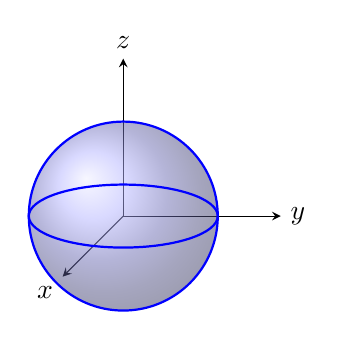
\begin{tikzpicture}[>=stealth, scale=1]
    % Assi 
    \draw[->] (0,0,0) -- (0,0,2) node[below left] {$x$};
    \draw[->] (0,0,0) -- (2,0,0) node[right] {$y$};
    \draw[->] (0,0,0) -- (0,2,0) node[above] {$z$};
    
    % Sfera (Rappresentazione densità)
    \shade[ball color=blue!40, opacity=0.5] (0,0,0) circle (1.2);
    \draw[blue, thick] (0,0,0) circle (1.2);
    % Meridiani/Paralleli per dare effetto 3D
    \draw[blue, thick] (0,0,0) ellipse (1.2 and 0.4);

\end{tikzpicture}
\caption{Orbitale \(s\) .}
\label{fig:orbitali_s}
\end{figure}

\vspace{0.5em}
\textbf{Orbitale $p$ ($\ell=1$)} \\
Per $\ell=1$, il numero quantico magnetico può essere $m_\ell = -1, 0, 1$. Le funzioni d'onda perdono la simmetria sferica e acquisiscono una dipendenza direzionale, manifestando dei \textbf{piani nodali} (piani in cui la probabilità di trovare l'elettrone è rigorosamente nulla, e che passano per il nucleo). 
Combinando linearmente le autofunzioni, si ottengono i tre orbitali reali orientati lungo i tre assi cartesiani ($p_x, p_y, p_z$), caratterizzati da una forma a "doppio lobo".

\begin{figure}[ht]
    \centering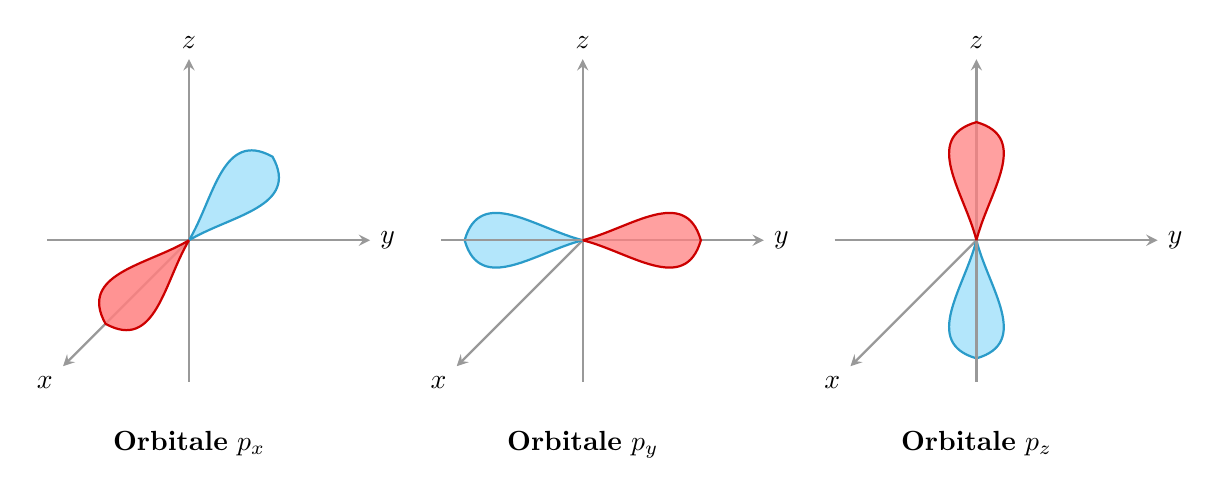
\begin{tikzpicture}[>=stealth, scale=1]

    % Assi lunghi 2.3 per superare i lobi (lunghi 1.5)
    \tikzset{asse/.style={->, thick, gray!80}}
    
    % Definizione della VERA forma a goccia quantistica (stretta al centro, larga in punta)
    \def\lobo{ (0,0) .. controls (0.15,0.6) and (0.7,1.3) .. (0,1.5) .. controls (-0.7,1.3) and (-0.15,0.6) .. (0,0) }

    % --- Orbitale p_x ---
    \begin{scope}[xshift=0cm]
        % Assi Y e Z
        \draw[asse] (-1.8,0) -- (2.3,0) node[right, text=black] {$y$};
        \draw[asse] (0,-1.8) -- (0,2.3) node[above, text=black] {$z$};

        % Lobo posteriore (fase -, azzurro) ruotato di 45 gradi (esattamente in asse con x in profondità)
        \begin{scope}[rotate around={-45:(0,0)}]
             \draw[draw=cyan!80!black, thick, fill=cyan!40, fill opacity=0.75] \lobo;
        \end{scope}

        % Asse X (A 225 gradi esatti, x=-1.4, y=-1.4)
        \draw[asse] (0,0) -- (-1.6,-1.6) node[below left, text=black] {$x$};

        % Lobo anteriore (fase +, rosso) ruotato di 225 gradi (esattamente lungo l'asse x visibile)
        \begin{scope}[rotate around={-225:(0,0)}]
             \draw[draw=red!80!black, thick, fill=red!50, fill opacity=0.85] \lobo;
        \end{scope}
        
        \node[below=2.3cm] {\textbf{Orbitale} $\boldsymbol{p_x}$};
    \end{scope}

    % --- Orbitale p_y ---
    \begin{scope}[xshift=5cm]
        % Asse Z e X
        \draw[asse] (0,-1.8) -- (0,2.3) node[above, text=black] {$z$};
        \draw[asse] (0,0) -- (-1.6,-1.6) node[below left, text=black] {$x$};

        % Lobo sinistro (fase -, azzurro) sull'asse y negativo (+90 gradi)
        \begin{scope}[rotate around={90:(0,0)}]
             \draw[draw=cyan!80!black, thick, fill=cyan!40, fill opacity=0.75] \lobo;
        \end{scope}

        % Asse Y
        \draw[asse] (-1.8,0) -- (2.3,0) node[right, text=black] {$y$};

        % Lobo destro (fase +, rosso) sull'asse y positivo (-90 gradi)
        \begin{scope}[rotate around={-90:(0,0)}]
             \draw[draw=red!80!black, thick, fill=red!50, fill opacity=0.75] \lobo;
        \end{scope}
        
        \node[below=2.3cm] {\textbf{Orbitale} $\boldsymbol{p_y}$};
    \end{scope}

    % --- Orbitale p_z ---
    \begin{scope}[xshift=10cm]
        % Assi X e Y
        \draw[asse] (-1.8,0) -- (2.3,0) node[right, text=black] {$y$};
        \draw[asse] (0,0) -- (-1.6,-1.6) node[below left, text=black] {$x$};

        % Lobo inferiore (fase -, azzurro) sull'asse z negativo (+180 gradi)
        \begin{scope}[rotate around={180:(0,0)}]
             \draw[draw=cyan!80!black, thick, fill=cyan!40, fill opacity=0.75] \lobo;
        \end{scope}

        % Asse Z
        \draw[asse] (0,-1.8) -- (0,2.3) node[above, text=black] {$z$};

        % Lobo superiore (fase +, rosso) sull'asse z positivo (0 gradi)
        \begin{scope}[rotate around={0:(0,0)}]
             \draw[draw=red!80!black, thick, fill=red!50, fill opacity=0.75] \lobo;
        \end{scope}
        
        \node[below=2.3cm] {\textbf{Orbitale} $\boldsymbol{p_z}$};
    \end{scope}

\end{tikzpicture}
\caption{Orbitali \(p_x, \,p_y,\,p_z\) .}
    \label{fig:orbitali_p}
\end{figure}

\lezione{2}{24/02/2026}

Abbiamo già detto che nell'atomo di idrogeno l'energia dipende solo da \(n\) e vale:
\begin{equation}
    E^{(0)}_n = -\frac12 \mu c^2 \frac{(Z\alpha)^2}{n^2}
\end{equation}
dove \(\alpha= \frac{e^2}{4\pi \epsilon_0\hbar c } \simeq \frac{1}{137}\) è la costante di struttura fine.
Considerando la molteplicità dello spin, il numero di autostati di energia \(E_n\) sarà:
\begin{equation}
    2 \sum_{\ell=0}^{n-1}(2\ell+1)= 2n^2
\end{equation} 

\begin{definition}
    Chiamiamo \textbf{shell} l'insieme di autostati con medesimo numero quantico principale \(n\) e \textbf{subshell} l'insieme di autostati con medesimo numero quantico principale \(n\) e numero quantico orbitale \(\ell\).\\
    Diremo inoltre che una shell (o una subshell) è \textbf{chiusa} quando ospita il numero massimo di elettroni che le compete.
\end{definition}
Il modelllo dell'atomo idrogenoide funziona bene anche per atomi con più elettroni, ma solo uno nella shell più esterna. 
Le shell interne sono chiuse e schermano la carica del nucleo, andraà dunque considerata solo la \textbf{carica efficace} del nucleo.


\subsection{Correzioni}
L'espressione di \(H^{(0)}\) non tiene conto del fatto che l'elettrone è una particella relativistica dotata di spin e, infatti,
lo studio degli spettri di emissione e assorbimento degli atomi idrogenoidi non è pienamente soddisfacente,
specialmente per giustificare la presenza di multipletti.

\subsubsection{Correzione di Darwin}
Il primo termine correttivo da considerare è la \textbf{correzione di Darwin} \(\Delta H_D\):
\begin{equation}
    \Delta H_D = \frac{\pi \hbar^2}{2m_e^2 c^2} \frac{Ze^2}{4\pi \epsilon_0}\delta_D(\vec{r})
\end{equation} 
Questa è una correzione di natura puramente quantistica che può essere spiegata come effetto del principio di indeterminazione.
Il valore medio per un certo autostato \(\ket{n,\ell,m_\ell, m_s}\):
\begin{equation}
    \expval{\Delta H_D} = \frac{\hbar^2}{2m_e c^2}  \frac{Z^4e^2}{4\pi \epsilon_0 a_0n^3}
\end{equation}
che scala come \(Z^4\) e \(\frac{1}{n^3}\). 

\subsubsection{Correzione relativistica}
Espressione relativistica dell'energia cinetica:
\begin{equation}
    E = \sqrt{p^2 c^2 + m_e^2 c^4} \qquad T = E - m_e c^2
\end{equation}

\begin{remark}
    In SR LAB vale questa. In SR CM metto $\mu$ al posto di $m_e$ ma $\mu \approx m_e$, quindi è come stare nel LAB.
\end{remark}

Come riscriviamo $T$ ora:
\begin{align*}
    T &= E - m_e c^2 = \left\{ \sqrt{p^2 c^2 + m_e^2 c^4} - m_e c^2 \right\} = \\[1ex]
      &= m_e c^2 \left\{ \sqrt{\frac{p^2 c^2}{m_e^2 c^4} + 1} - 1 \right\} = m_e c^2 \left\{ \sqrt{\frac{p^2}{m_e^2 c^2} + 1} - 1 \right\} \approx \text{espandiamo} \approx \\[1ex]
      &\approx m_e c^2 \left\{ \cancel{1} + \frac{1}{2}\frac{p^2}{m_e^2 c^2} - \frac{1}{8}\frac{p^4}{m_e^4 c^4} + \dots - \cancel{1} \right\}
\end{align*}
Otteniamo dunque:
\begin{equation}
    \Delta H_{rel} = - \frac{p^4}{8m_e^3c^2}
\end{equation}

L'ordine di grandezza risulta:
\begin{equation}
    \frac{\expval{\Delta H_{rel}}}{\expval{T}} \sim \frac{1}{4} \left( \frac{v}{c} \right)^2 \sim 10^{-4}
\end{equation}
Sarà rilevante dunque solo in apparati ad alta risoluzione.

\subsubsection{Interazione Spin-orbita}

L'interazione tra l'elettrone ($e^-$) e il campo elettrico $\vec{E}$ generato dal nucleo viene percepita come un campo magnetico $\vec{B}$ dall'elettrone stesso.

Nel sistema di riferimento del laboratorio (SR LAB), considerando il nucleo con carica $Ze$, il campo elettrico generato è dato da:
\begin{equation}
    \vec{E} = \frac{Ze}{4\pi\varepsilon_0 r^2} \hat{u}_r = \frac{Ze}{4\pi\varepsilon_0 r^3} \vec{r}
\end{equation}

Poiché l'elettrone è in moto rispetto al sistema del laboratorio, dobbiamo effettuare le trasformazioni di Lorentz per passare al sistema di riferimento solidale all'elettrone (SR $e^-$). In questo nuovo sistema, descritto dagli assi $(x', y', z')$, l'elettrone agisce come una carica di prova $-e$ posta nell'origine.

Nel limite non relativistico, ovvero assumendo $\abs{\frac{\vec{v}}{c}} \ll 1$, il campo magnetico $\vec{B}'$ ``visto'' nel sistema di riferimento $x', y', z'$ è dovuto alla trasformazione di Lorentz del campo elettrico $\vec{E}$ e si approssima a:
\begin{equation}
    \vec{B}' \simeq -\frac{\vec{v}}{c^2} \wedge \vec{E} = -\frac{\vec{v}}{c^2} \wedge \frac{Ze}{4\pi\varepsilon_0 r^3} \vec{r}
\end{equation}
dove $\vec{r}$ è il vettore posizione che va dal nucleo all'elettrone.

Sviluppando l'espressione del campo magnetico e raccogliendo i termini, possiamo evidenziare la dipendenza dal momento angolare dell'elettrone:
\begin{equation}
    \vec{B}' = \underbrace{\frac{Ze}{4\pi\varepsilon_0 r^3 m_e c^2}}_{:= K_Z(r)} (\vec{r} \wedge m_e \vec{v})
\end{equation}
Il termine $(\vec{r} \wedge m_e \vec{v})$ rappresenta proprio il momento angolare orbitale dell'elettrone, che indichiamo con $\vec{L}$. Il fattore scalare $K_Z(r)$ definisce l'intensità dell'interazione in funzione della distanza e del nucleo; in particolare, si osserva una dipendenza lineare dal numero atomico ($K_Z(r) \propto Z$) e inversamente proporzionale al cubo della distanza ($K_Z(r) \propto \frac{1}{r^3}$). 

Possiamo quindi riscrivere il campo magnetico in forma compatta come:
\begin{equation}
    \vec{B}' = K_Z(r) \vec{L}
\end{equation}

Questo campo $\vec{B}'$ ha un effetto fisico rilevante: lo spin dell'elettrone interagisce con esso, dando origine a un moto di precessione. L'interazione si manifesta attraverso un momento torcente (o meccanico) $\vec{M}$ applicato sull'elettrone, dato da:
\begin{equation}
    \vec{M} = \vec{\mu}_s \wedge \vec{B}'
\end{equation}
dove $\vec{\mu}_s$ rappresenta il momento magnetico di spin. 

Ricordiamo che il momento magnetico di spin è direttamente proporzionale al vettore spin $\vec{s}$ tramite la relazione:
\begin{equation}
    \vec{\mu}_s = -g_s \frac{\mu_B}{\hbar} \vec{S}
\end{equation}
in cui $g_s \simeq 2,0$ è il fattore giromagnetico di spin dell'elettrone e $\mu_B$ è il magnetone di Bohr.
La correzione all'Hamiltoniana derivante dall'interazione spin-orbita è costituita, in prima battuta, dall'energia di interazione associata al dipolo magnetico immerso nel campo $\vec{B}'$:
\begin{equation}
    \Delta H_{\text{int } \vec{B}'-\vec{s}} = - \vec{\mu}_s \cdot \vec{B}'
\end{equation}

Sostituendo le espressioni precedentemente ricavate per il momento magnetico di spin ($\vec{\mu}_s$) e per il campo magnetico ($\vec{B}'$), i segni meno si elidono e otteniamo:
\begin{equation}
    \Delta H_{\text{int } \vec{B}'-\vec{s}} = + g_s \frac{\mu_B}{\hbar} K_Z(r) (\vec{S} \cdot \vec{L})
\end{equation}
Come si evince dall'equazione, questo termine correttivo risulta direttamente proporzionale al prodotto scalare $\vec{S} \cdot \vec{L}$, motivo per cui tale effetto prende il nome di interazione ``spin-orbita''.

Tuttavia, questa trattazione preliminare non è sufficiente come correzione esatta del sistema. Per una descrizione cinematica corretta, bisogna affiancare al sistema di riferimento del laboratorio (SR LAB) e a quello traslante solidale all'elettrone (SR $e^-$, definito dagli assi $x', y', z'$ centrati in $O'$ e in moto a velocità $\vec{v}_{e^-}$) un ulteriore sistema di riferimento. Si definisce quindi un nuovo sistema di assi $x'', y'', z''$, anch'esso centrato in $O'$, ma che ruota con una velocità angolare $\vec{\omega}'$ rispetto al sistema intermedio $x', y', z'$. L'elettrone, pertanto, si trova in un sistema che non solo si muove a velocità $\vec{v}_{e^-}$, ma che contemporaneamente ruota.

Nel sistema di riferimento del laboratorio ($x,y,z$), si dimostra che la velocità angolare di rotazione $\vec{\omega}'$ assume la forma della cosiddetta velocità angolare di Thomas, che denotiamo con $\vec{\omega}_T$:
\begin{equation}
    \vec{\omega}_T = \frac{1}{2} \frac{\vec{a} \wedge \vec{v}_e}{c^2} = \frac{1}{2c^2} \left( -\frac{e\vec{E}}{m_e} \wedge \vec{v}_e \right)
\end{equation}
dove $\vec{v}_e$ è la velocità dell'elettrone rispetto al sistema di riferimento del laboratorio e $\vec{a}$ è l'accelerazione derivante dall'interazione coulombiana. Dato che stiamo considerando un atomo idrogenoide, possiamo usare l'equazione del moto $m_e \vec{a} = -e\vec{E}$.

Sostituendo l'espressione del campo elettrico e moltiplicando e dividendo per la massa dell'elettrone $m_e$, possiamo evidenziare il termine relativo al momento angolare orbitale $\vec{L} = \vec{r} \wedge m_e \vec{v}_e$:
\begin{equation}
    \vec{\omega}_T = - \frac{1}{2c^2} \frac{Ze^2}{4\pi\varepsilon_0 r^3 m_e} \frac{(\vec{r} \wedge m_e \vec{v}_e)}{m_e} = - \frac{1}{2} K_Z(r) \vec{L} \frac{e}{m_e}
\end{equation}

In sintesi, l'elettrone possiede un grado di libertà interno (lo spin) che manifesta proprietà analoghe a quelle di una particella dotata di momento angolare intrinseco $\vec{s}$ e momento magnetico di spin $\vec{\mu}_s$. 
Questo interagisce con il nucleo in un modo complesso. Una prima complessità deriva direttamente dal moto orbitale: l'elettrone "sente" il campo $\vec{E}$ nucleare, che nel suo sistema di riferimento diventa un campo $\vec{B}'$; questo campo magnetico, a sua volta, interferisce con lo spin. 
Si tratta a tutti gli effetti di un fenomeno autoindotto in cui $\vec{L}$ interagisce con $\vec{S}$.

Abbiamo, dunque, che la cinematica del sistema rotante introduce un'ulteriore correzione energetica connessa all'interazione spin-orbita:
\begin{equation}
    \Delta H_{\text{sist. rotante - spin}} = \vec{\omega}_T \cdot \vec{S} = - \frac{1}{2} K_Z(r) \left(\vec{L} \cdot \vec{S}\right) \frac{e}{m_e}
\end{equation}

Chiameremo più propriamente correzione (complessiva) di \text{SPIN-ORBITA}:
\begin{align}
    \Delta H_{SO} &= \Delta H_{in, \vec{B}' \cdot \vec{S}} + \Delta H_{sist. rotante - spin} = \nonumber \\
    &= \frac{e}{m_e} \left( K_z(r) \vec{L} \cdot \vec{S} - \frac{1}{2} K_z(r) \vec{L} \cdot \vec{S} \right) =\frac{e}{m_e} \frac{1}{2} K_z(r) \vec{L} \cdot \vec{S} = \xi_z(r) \vec{L} \cdot \vec{S}
\end{align}

Calcoliamo quanto vale il valore aspettazione per un generico autostato di \(H^{(0)}\), ovvero \(R_{n\ell}(r) Y_\ell^{m_\ell}(\theta, \phi) \chi_{s, m_s}\) che descriviamo com il ket \(\ket{n, \ell, m_\ell, s, m_s}\):
\begin{equation*}
    \expval{\Delta H_{SO}} = \mel{n, \ell, m_\ell, s, m_s}{\xi_z(r)\vec{L} \cdot \vec{S}}{n, \ell, m_\ell, s, m_s}
\end{equation*}
Tuttavia, la presenza del termine $\vec{L} \cdot \vec{S}$ mescola gli autostati di $H^{(0)}$, per cui è necessario effettuare un cambio di base. \\
Usiamo il momento angolare totale $\vec{J} = \vec{L} + \vec{S}$ associato all'operatore $\vec{J}$:
\begin{equation}
    \begin{cases}
        J^2 \ket{j, m_j} = \hbar^2 j(j+1) \ket{j, m_j} \\
        J_z \ket{j, m_j} = \hbar m_j \ket{j, m_j}
    \end{cases}
\end{equation}
Sulla base O.N. \(\ket{j,m_j}\), tale che soddisfi queste condizioni:

\begin{equation}
    m_j = \underbrace{-j, -j+1, \dots, j}_{2j+1} \qquad \qquad \abs{\ell - s} \le j \le \ell + s
\end{equation}

Dato \(\vec{S} \) e \( \vec{L}\) commutano abbiamo che:
\begin{equation}
    \vec{J} = \vec{S} + \vec{L} \implies J^2 = S^2 + L^2 + 2 \vec{S} \cdot \vec{L} 
\end{equation}

\begin{equation}
    \vec{S} \cdot \vec{L} = \frac{J^2 - S^2 - L^2}{2}
    \implies \Delta H_{SO} = \xi_z(r) \vec{L} \cdot \vec{S} = \xi_z(r) \left\{ \frac{J^2 - L^2 - S^2}{2} \right\} 
\end{equation}

\begin{equation}
    \label{eq: expval_Hso}
    \mel{j, m_j}{\Delta H_{SO}}{j, m_j} = \mel{j, m_j}{\xi(r)}{j, m_j} \cdot \hbar^2 \left\{ \frac{j(j+1) - \ell(\ell+1) - s(s+1)}{2} \right\}
\end{equation}

\lezione{3}{02/03/2026}

Ricordiamo che gli autostati della base \(\left\{ \ket{j,m_j} \right\}\) (dove sono impiciti gli autovalori \(n, \ell, s\)) 
possono essere ottenuti dalla base di autostati di \(H^{(0)}\) \(\left\{ \ket{n, \ell, m_{\ell}, s, m_s} \right\}\) mediante i coefficienti di Clebsch-Gordan:

\begin{equation}
    \ket{j, m_j} = \sum_{m_{\ell}=-\ell}^{\ell} \sum_{m_s=-s}^{s} \underbrace{\braket{n, \ell, m_{\ell}, s, m_s}{j, m_j}}_{\text{coeff. Clebsch-Gordan}} \ket{n, \ell, m_{\ell},s , m_s}
\end{equation}

dove gli stati \(\ket{n, \ell, m_{\ell}, s, m_s}\) sono associati alle funzioni d'onda \( R_{n,\ell}(r) Y_{\ell}^{m_{\ell}}(\theta,\phi) \chi_{s,m_s}\) .

Sapendo che \(\xi(r) \propto \frac{1}{r^3}\), possiamo risolvere dunque l'equazione \ref{eq: expval_Hso} 
calcolando il valore di aspettazione di $\frac{1}{r^3}$ sullo stato $\ket{j, m_j}$. 
L'integrale si riduce alle sole coordinate spaziali, la parte di spin, infatti, restituisce $1$ quando proiettata su se stessa:

\begin{equation}
    \mel{j, m_j}{\frac{1}{r^3}}{j, m_j} = (\dots) \int_0^\infty \frac{r^2}{r^3} \abs{R_{n,\ell}(r)}^2 \, dr \underbrace{\int_{\Omega} \abs{Y_{\ell}^{m_{\ell}}(\theta,\phi)}^2 \sin\theta \, d\theta \, d\phi}_{\text{integrale sull'angolo solido}}
\end{equation}

L'integrale radiale appena ricavato è un risultato noto per le autofunzioni dell'Hamiltoniana imperturbata $H^{(0)}$ di un atomo idrogenoide:

\begin{equation}
    \underbrace{\mel{n, \ell, m_{\ell}, s, m_s}{\frac{1}{r^3}}{n, \ell, m_{\ell}, s, m_s}}_{\text{autofunz. di } H^{(0)}} = \frac{2}{a^3 n^3 \ell(\ell+1)(2\ell+1)} \qquad \text{con} \quad a = \frac{4\pi \varepsilon_0 \hbar^2}{Z e^2 \mu}
\end{equation}

Con questo risultato in mente, calcolando l'elemento di matrice dell'operatore di spin-orbita, si ricava la correzione energetica $\Delta E_{SO}$:

\begin{equation}
    \mel{j, m_j}{\Delta H_{SO}}{j, m_j} = Z^4 \alpha^4 \frac{m_e c^2}{2} \frac{1}{n^3} \frac{j(j+1) - \ell(\ell+1) - s(s+1)}{\ell(\ell+1)(2\ell+1)}
\end{equation}
La variazione di energia \(\Delta E_{SO}\) è proporzionale a \(Z^4\) e \(\frac{1}{n^3}\) .

\begin{attention}
    Questo risultato vale esclusivamente per $\ell \neq 0$. È importante notare che per $\ell = 0$ il termine di spin-orbita è nullo e la trattazione richiede considerazioni differenti (come il termine di Darwin).
\end{attention}

\subsubsection{Splitting energetici}

La correzione dipende in modo non banale dai numeri quantici. In particolare, il termine di interazione spin-orbita \( \Delta E_{SO} \) dipende dai numeri quantici \( j \), \( \ell \) e \( s \).

Per un atomo idrogenoide, dove lo spin dell'elettrone è \( s = \frac{1}{2} \), i valori possibili per il numero quantico del momento angolare totale sono vincolati dalla relazione:
\begin{equation}
    |\ell - s| \le j \le \ell + s \implies j = \ell \pm \frac{1}{2}
\end{equation}

Valutando il termine accoppiamento \( j(j+1) - \ell(\ell+1) - s(s+1) \) nei due casi possibili, otteniamo:
\begin{itemize}
    \item Se \( j = \ell + \frac{1}{2} \):
    \[ j(j+1) - \ell(\ell+1) - s(s+1) = \ell \]
    \item Se \( j = \ell - \frac{1}{2} \):
    \[ j(j+1) - \ell(\ell+1) - s(s+1) = -\ell - 1 \]
\end{itemize}

L'interazione tra il momento angolare orbitale \( \ell \) e lo spin \( s \) rimuove la degenerazione dei livelli energetici dell'Hamiltoniana imperturbata \( H^{(0)} \). 
A partire dallo stato \( E^{(0)} \), si osserva uno \textbf{splitting}: una separazione degli stati con conseguente rimozione della degenerazione spaziale.

\begin{figure}[htbp]
    \centering
    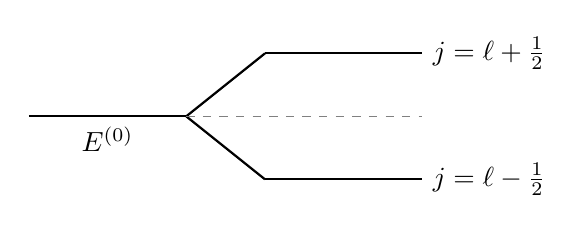
\begin{tikzpicture}[node distance=2cm, thick]
        % Livello imperturbato
        \draw (0,0) -- (2,0) node[midway, below] {\( E^{(0)} \)};
        
        % Linee di splitting (diagonali)
        \draw (2,0) -- (3,0.8);
        \draw (2,0) -- (3,-0.8);
        
        % Livelli splittati (orizzontali)
        \draw (3,0.8) -- (5,0.8) node[right] {\( j = \ell + \frac{1}{2} \)};
        \draw (3,-0.8) -- (5,-0.8) node[right] {\( j = \ell - \frac{1}{2} \)};
        
        % Opzionale: tratteggio per evidenziare lo spostamento
        \draw[dashed, thin, gray] (2,0) -- (5,0);
    \end{tikzpicture}
    \caption{Splitting energetico dall'interazione SO}
\end{figure}


L'energia \( E^{(0)} \) vale:
\begin{equation}
    E^{(0)} := \frac{\alpha^2 m_e c^2}{2} \simeq 13.6 \text{ eV}
\end{equation}
Questa quantità rappresenta l'energia necessaria per estrarre un elettrone dall'atomo e portarlo a distanza infinita, ovvero l'energia di prima ionizzazione. 

L'espressione per la variazione di energia dovuta all'interazione spin-orbita (che costituisce una parte delle correzioni relativistiche) è:
\begin{equation}
    \Delta E_{SO} = Z^4 \alpha^2 \frac{E^{(0)}}{n^3} \frac{j(j+1) - \ell(\ell+1) - s(s+1)}{\ell(\ell+1)(2\ell+1)}
\end{equation}
Sostituendo il termine dipendente dai numeri quantici calcolato in precedenza, possiamo distinguere i due casi possibili per \( j \):
\begin{equation}
    \Delta E_{SO|j=\ell+\frac{1}{2}} = \frac{Z^4 \alpha^2 E^{(0)}}{n^3 (\ell+1)(2\ell+1)} \quad 
    \Delta E_{SO|j=\ell-\frac{1}{2}} = - \frac{Z^4 \alpha^2 E^{(0)}}{n^3 \ell(2\ell+1)} 
\end{equation}


A partire da un singolo livello degenere, la correzione di spin-orbita rimuove parzialmente la degenerazione La separazione dei livelli porta alla formazione di un \textbf{doppietto}.
\begin{remark}
    La correzione \(\Delta E_{SO}\) è di modesta entità: \( 10^{-5} \divisionsymbol 10^{-3} \;eV\) .
\end{remark}

\begin{attention}
    È fondamentale sottolineare che questa perturbazione \emph{non} rimuove la degenerazione spaziale legata all'orientazione. Ogni stato splittato mantiene una degenerazione associata al numero quantico \( m_j \) (o \( m_\ell \)), che rimane inalterata.
\end{attention}


\subsubsection{Shifting}

Lo \textbf{shifting} rappresenta la variazione di energia tra un singolo sottolivello del multipletto e l'energia imperturbata del sistema.

\begin{figure}[htbp]
\centering
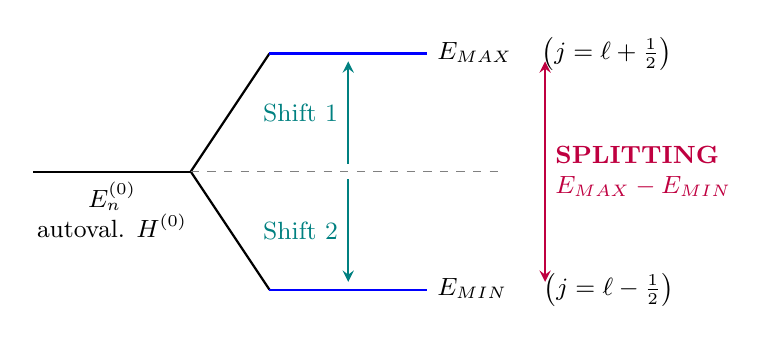
\begin{tikzpicture}[thick, font=\small]
    % Livello imperturbato di partenza
    \draw (0,0) -- (2,0) node[midway, below, align=center] {\( E_n^{(0)} \) \\ autoval. \( H^{(0)} \)};
    
    % Linee di separazione
    \draw (2,0) -- (3,1.5);
    \draw (2,0) -- (3,-1.5);
    
    % Linea di riferimento centrale (continuazione del livello imperturbato)
    \draw[dashed, thin, gray] (2,0) -- (6,0);
    
    % Livelli splittati (Doppietto)
    \draw[blue] (3,1.5) -- (5,1.5) node[right, text=black] {\( E_{\text{MAX}} \quad \left(j = \ell + \frac{1}{2}\right) \)};
    \draw[blue] (3,-1.5) -- (5,-1.5) node[right, text=black] {\( E_{\text{MIN}} \;\quad \left(j = \ell - \frac{1}{2}\right) \)};
    
    % Indicazione dello Splitting (freccia a destra)
    \draw[<->, purple, >=stealth] (6.5, -1.4) -- (6.5, 1.4) node[midway, right, align=left] {\textbf{SPLITTING} \\ \( E_{\text{MAX}} - E_{\text{MIN}} \)};
    
    % Indicazioni dello Shifting (frecce interne)
    \draw[->, teal, >=stealth] (4, 0.1) -- (4, 1.4) node[midway, left] {Shift 1};
    \draw[->, teal, >=stealth] (4, -0.1) -- (4, -1.4) node[midway, left] {Shift 2};

\end{tikzpicture}
\caption{Shifting nel caso di doppietto}
\end{figure}

Lo shift è calcolato rispetto agli autovalori imperturbati \( H^{(0)} \). 
Pertanto, esso è definito come la differenza di energia tra il singolo sottolivello del multipletto e il valore corrispondente dell'autovalore imperturbato dell'Hamiltoniana \( H^{(0)} \).
    
In caso di multipletti si usa il termine shift per indicare la differenza di energia di due sottolivelli consecutivi.

\begin{figure}[htbp]
    \centering
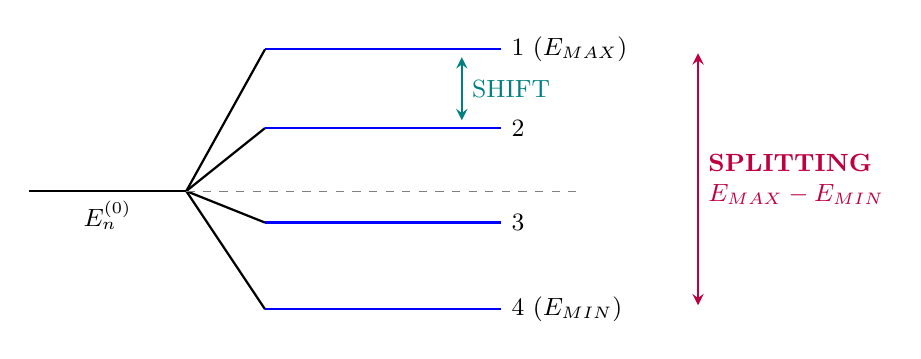
\begin{tikzpicture}[thick, font=\small]
    % Livello imperturbato di partenza
    \draw (0,0) -- (2,0) node[midway, below, align=center] {\( E_n^{(0)} \)};
    
    % Linee di separazione (Splitting) verso il multipletto
    \draw (2,0) -- (3, 1.8);
    \draw (2,0) -- (3, 0.8);
    \draw (2,0) -- (3, -0.4);
    \draw (2,0) -- (3, -1.5);
    
    % Linea di riferimento centrale
    \draw[dashed, thin, gray] (2,0) -- (7,0);
    
    % Livelli del multipletto (Sottolivelli 1, 2, 3, 4)
    \draw[blue] (3, 1.8) -- (6, 1.8) node[right, text=black] {1 (\( E_{\text{MAX}} \))};
    \draw[blue] (3, 0.8) -- (6, 0.8) node[right, text=black] {2};
    \draw[blue] (3,-0.4) -- (6,-0.4) node[right, text=black] {3};
    \draw[blue] (3,-1.5) -- (6,-1.5) node[right, text=black] {4 (\( E_{\text{MIN}} \))};
    
    % Indicazione dello SHIFT (tra 2 valori consecutivi)
    \draw[<->, teal, >=stealth] (5.5, 0.9) -- (5.5, 1.7) node[midway, right] {SHIFT};
    
    % Indicazione dello SPLITTING (tra MAX e MIN)
    \draw[<->, purple, >=stealth] (8.5, -1.45) -- (8.5, 1.75) node[midway, right, align=left] {\textbf{SPLITTING} \\ \( E_{\text{MAX}} - E_{\text{MIN}} \)};
    
\end{tikzpicture}
\caption{Shifting nel caso di multipletto}
\end{figure}


\begin{exercise}
    Calcoliamo lo splitting indotto dall'interazione \( S-O \) per \( n=2 \), \( \ell=1 \), in funzione di \( Z \), e successivamente per \( Z=1 \).

\begin{solution}

Per \( n=2 \) i valori possibili sono \( \ell=0, 1 \). In questo caso specifico consideriamo \( \ell=1 \) (orbitale di tipo \( p \)).

L'energia imperturbata al secondo livello è:
\begin{equation}
    E_2^{(0)} = -\frac{1}{2} \mu c^2 \frac{(Z\alpha)^2}{n^2} = -\frac{1}{8} \mu c^2 Z^2 \alpha^2
\end{equation}

Calcoliamo la correzione da aggiungere \(\Delta E_{SO \substack{n=2 \\ \ell=1}}\), 
dall'accoppiamento spin-orbita, per \( \ell=1 \), si ottengono i seguenti valori per il numero quantico \( j \):
\[
\ell=1 \longrightarrow j = 
\begin{cases} 
    \ell - \frac{1}{2} = \frac{1}{2} \\[1ex]
    \ell + \frac{1}{2} = \frac{3}{2} 
\end{cases}
\]

L'indicizzazione per i sottolivelli segue il \textbf{formalismo spettroscopico}:
\begin{equation}
    n ^{2s+1} \ell_j
\end{equation}
Dunque i due sottolivelli saranno indicati da \( 2^2 p_{\frac{1}{2}} \) e \( 2^2 p_\frac32 \) .

Per lo stato con momento angolare totale minimo \(2^2p_\frac12\), la correzione energetica è data da:
\[
    \Delta E_{SO}\eval_{j=1/2} = - \frac{Z^4 \alpha^2 E_0}{n^3 \ell(2\ell+1)}
    = - \frac{Z^4 \alpha^2 E_0}{2^3 \cdot 1(2 \cdot 1 + 1)} = - \frac{Z^4 \alpha^2 E_0}{24}
\]


Per lo stato con momento angolare totale massimo \(2^2p_{\frac32}\), la correzione è positiva (il livello si alza):
\[
    \Delta E_{SO}\eval_{j=3/2} = \frac{Z^4 \alpha^2 E_0}{n^3 (\ell+1)(2\ell+1)}
    = \frac{Z^4 \alpha^2 E_0}{2^3 (1+1)(2 \cdot 1 + 1)} = \frac{Z^4 \alpha^2 E_0}{48}
\]

Lo splitting energetico (\( \delta E_{SO} \)) sarà dunque:
\[
    \delta E_{SO} = E_{max} - E_{min} =  = \frac{Z^4 \alpha^2 E_0}{48} - \left( - \frac{Z^4 \alpha^2 E_0}{24} \right) = \frac{3 Z^4 \alpha^2 E_0}{48} = \frac{Z^4 \alpha^2 E_0}{16}
\]
Per l'atomo di Idrogeno (\( Z=1 \)), questo valore corrisponde a:
\[
    \delta E_{SO} \approx 4,5 \cdot 10^{-5} \text{ eV}
\]
\end{solution}
\end{exercise}

\subsubsection{Correzione complessiva}
\lezione{4}{03/03/2026}